% Salia sio .tex failo turi buti Mokinio_originalas.pdf.
% Mokinio sprendimai rodomi kaip originalaus PDF iskarpos, ne transkripcija.
\documentclass[11pt,a4paper]{article}
\usepackage[T1]{fontenc}
\usepackage[utf8]{inputenc}
\usepackage[lithuanian]{babel}
\usepackage{lmodern}
\usepackage{amsmath,amssymb}
\usepackage[a4paper,margin=1.8cm]{geometry}
\usepackage{enumitem}
\usepackage{xcolor}
\usepackage{fancyhdr}
\usepackage{microtype}
\usepackage{graphicx}
\definecolor{ink}{HTML}{203C50}
\setlength{\parindent}{0pt}
\setlength{\parskip}{4pt}
\setlist[itemize]{leftmargin=*,itemsep=3pt,topsep=3pt}
\setlength{\abovedisplayskip}{7pt}
\setlength{\belowdisplayskip}{7pt}
\pagestyle{fancy}
\fancyhf{}
\fancyhead[L]{\small Kvadratinių lygčių uždaviniai}
\fancyhead[R]{\small }
\fancyfoot[C]{\thepage}
\setlength{\headheight}{14pt}
\newcommand{\uzd}[2]{\begin{center}{\Large\bfseries\color{ink}#1 uždavinys}\end{center}\textbf{Sąlyga.} #2\par}
\newcommand{\dalis}[1]{\par\vspace{5pt}{\bfseries\color{ink}#1}\par}
\newcommand{\past}{\dalis{2. Pastabos mokiniui}}
\newcommand{\tais}{\dalis{3. Tvarkingas pataisytas sprendimas}}
\newcommand{\qed}{\hfill$\square$}
\begin{document}
\begin{center}
{\LARGE\bfseries Kvadratinių lygčių uždaviniai}\par
{\normalsize Pastabos ir patarimai}
\end{center}

\uzd{1}{Įrodykite, kad $x^2+(a+b)x+ab-c^2=0$ turi bent vieną realųjį sprendinį visiems $a,b,c\in\mathbb R$. Kada sprendinys vienintelis?}

\begin{center}
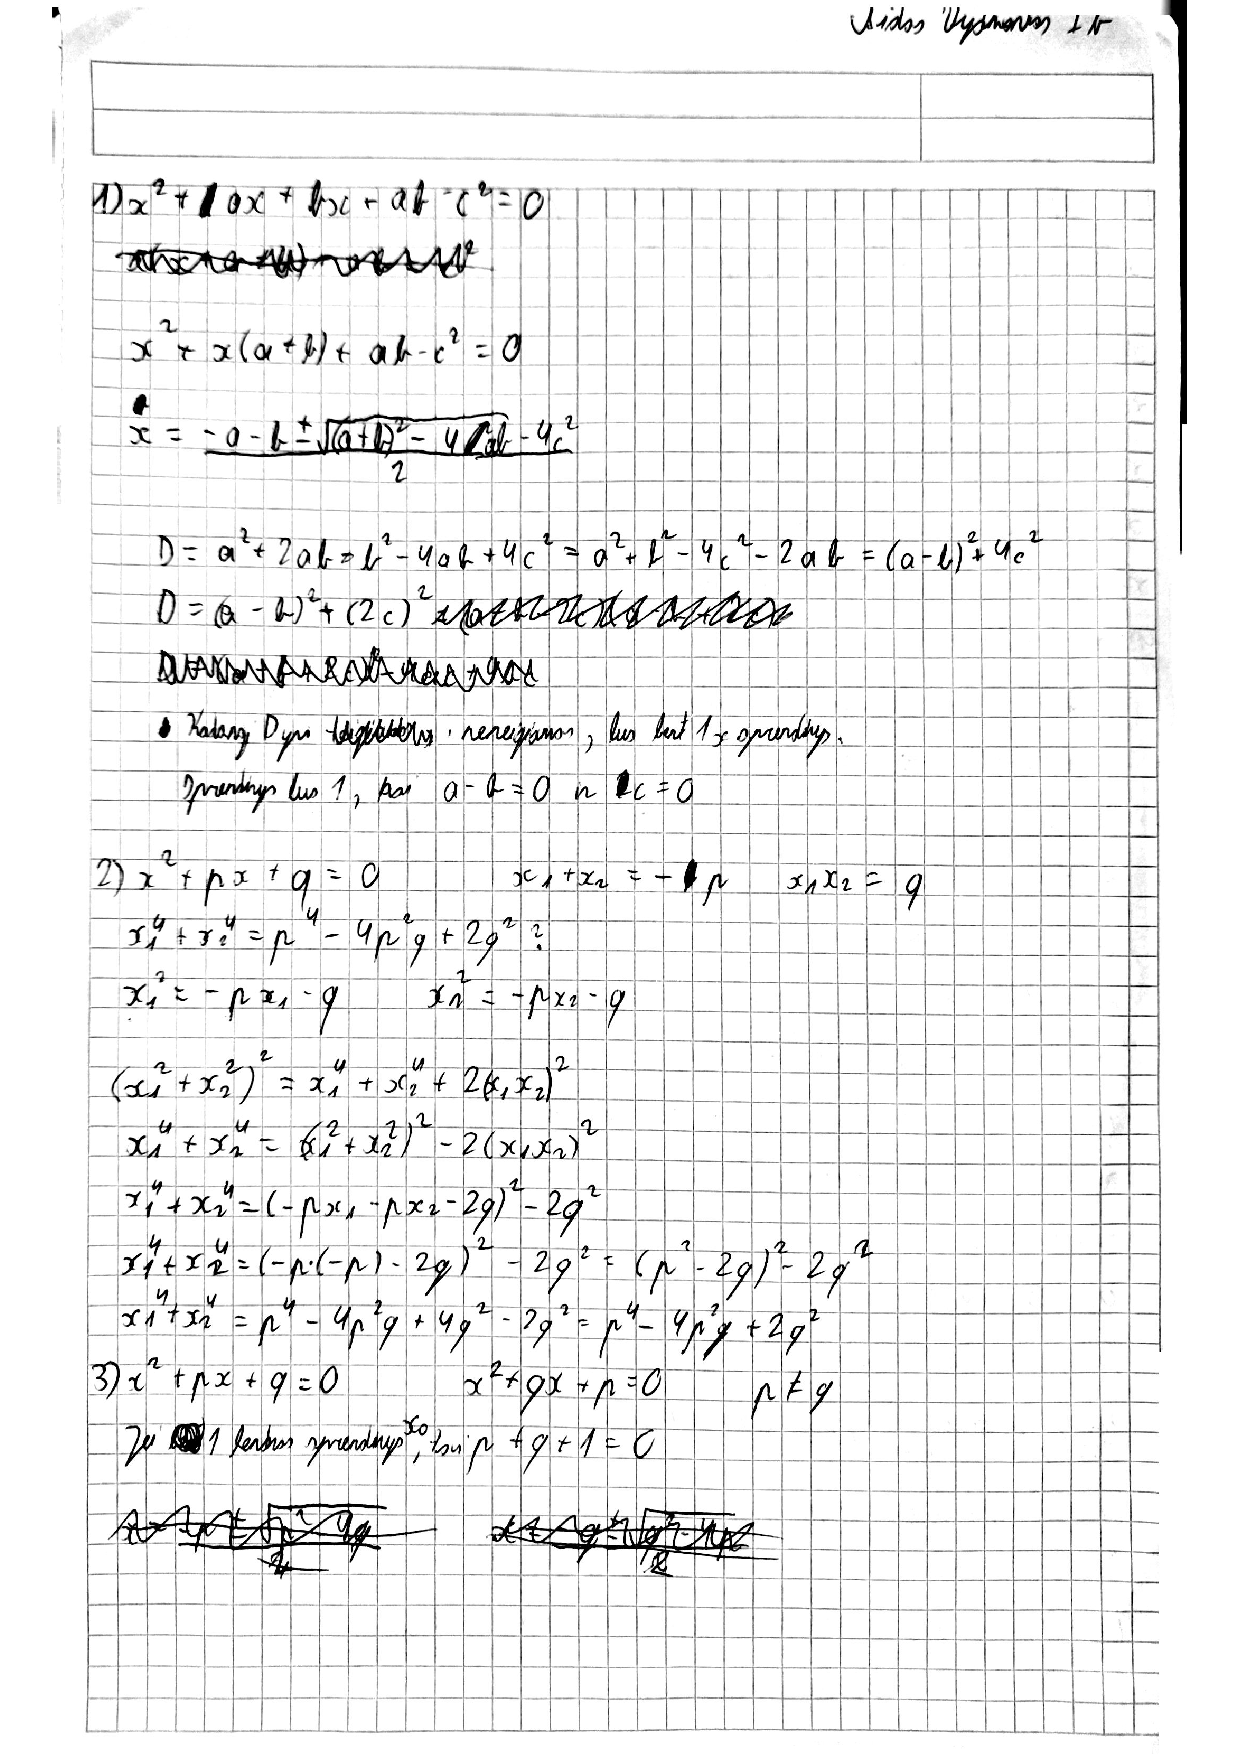
\includegraphics[page=1,trim={35.083 442.050 33.679 77.183},clip,width=\linewidth,height=.70\textheight,keepaspectratio]{Mokinio_originalas.pdf}\par
\end{center}
{\large\bfseries\color{ink}Pastabos ir pataisytas įrodymas}\par
\past
\begin{itemize}
\item Palikta aritmetinė klaida.
\end{itemize}
\tais
Lygties diskriminantas yra
\[
D=(a+b)^2-4(ab-c^2)
=a^2-2ab+b^2+4c^2=(a-b)^2+4c^2.
\]
Kadangi realiųjų skaičių kvadratai neneigiami, $D\ge0$. Kvadratinės lygties vyriausiasis koeficientas lygus $1\ne0$, todėl ji turi bent vieną realųjį sprendinį.

Lygtis turi lygiai vieną realųjį sprendinį tada, kai $D=0$. Neneigiamų dėmenų suma lygi nuliui tada, kai abu dėmenys lygūs nuliui. Todėl
\[
D=0\iff a-b=0\ \text{ir}\ c=0
\iff a=b\ \text{ir}\ c=0.
\]
Taigi vienintelis sprendinys yra būtent tada, kai $a=b$ ir $c=0$; tuo atveju lygtis yra $(x+a)^2=0$, o jos sprendinys $x=-a$.\qed

\newpage
\uzd{2}{Lygties $x^2+px+q=0$ sprendiniai yra $x_1,x_2$. Naudodamiesi Vijeto teorema įrodykite $x_1^4+x_2^4=p^4-4p^2q+2q^2$.}
\begin{center}
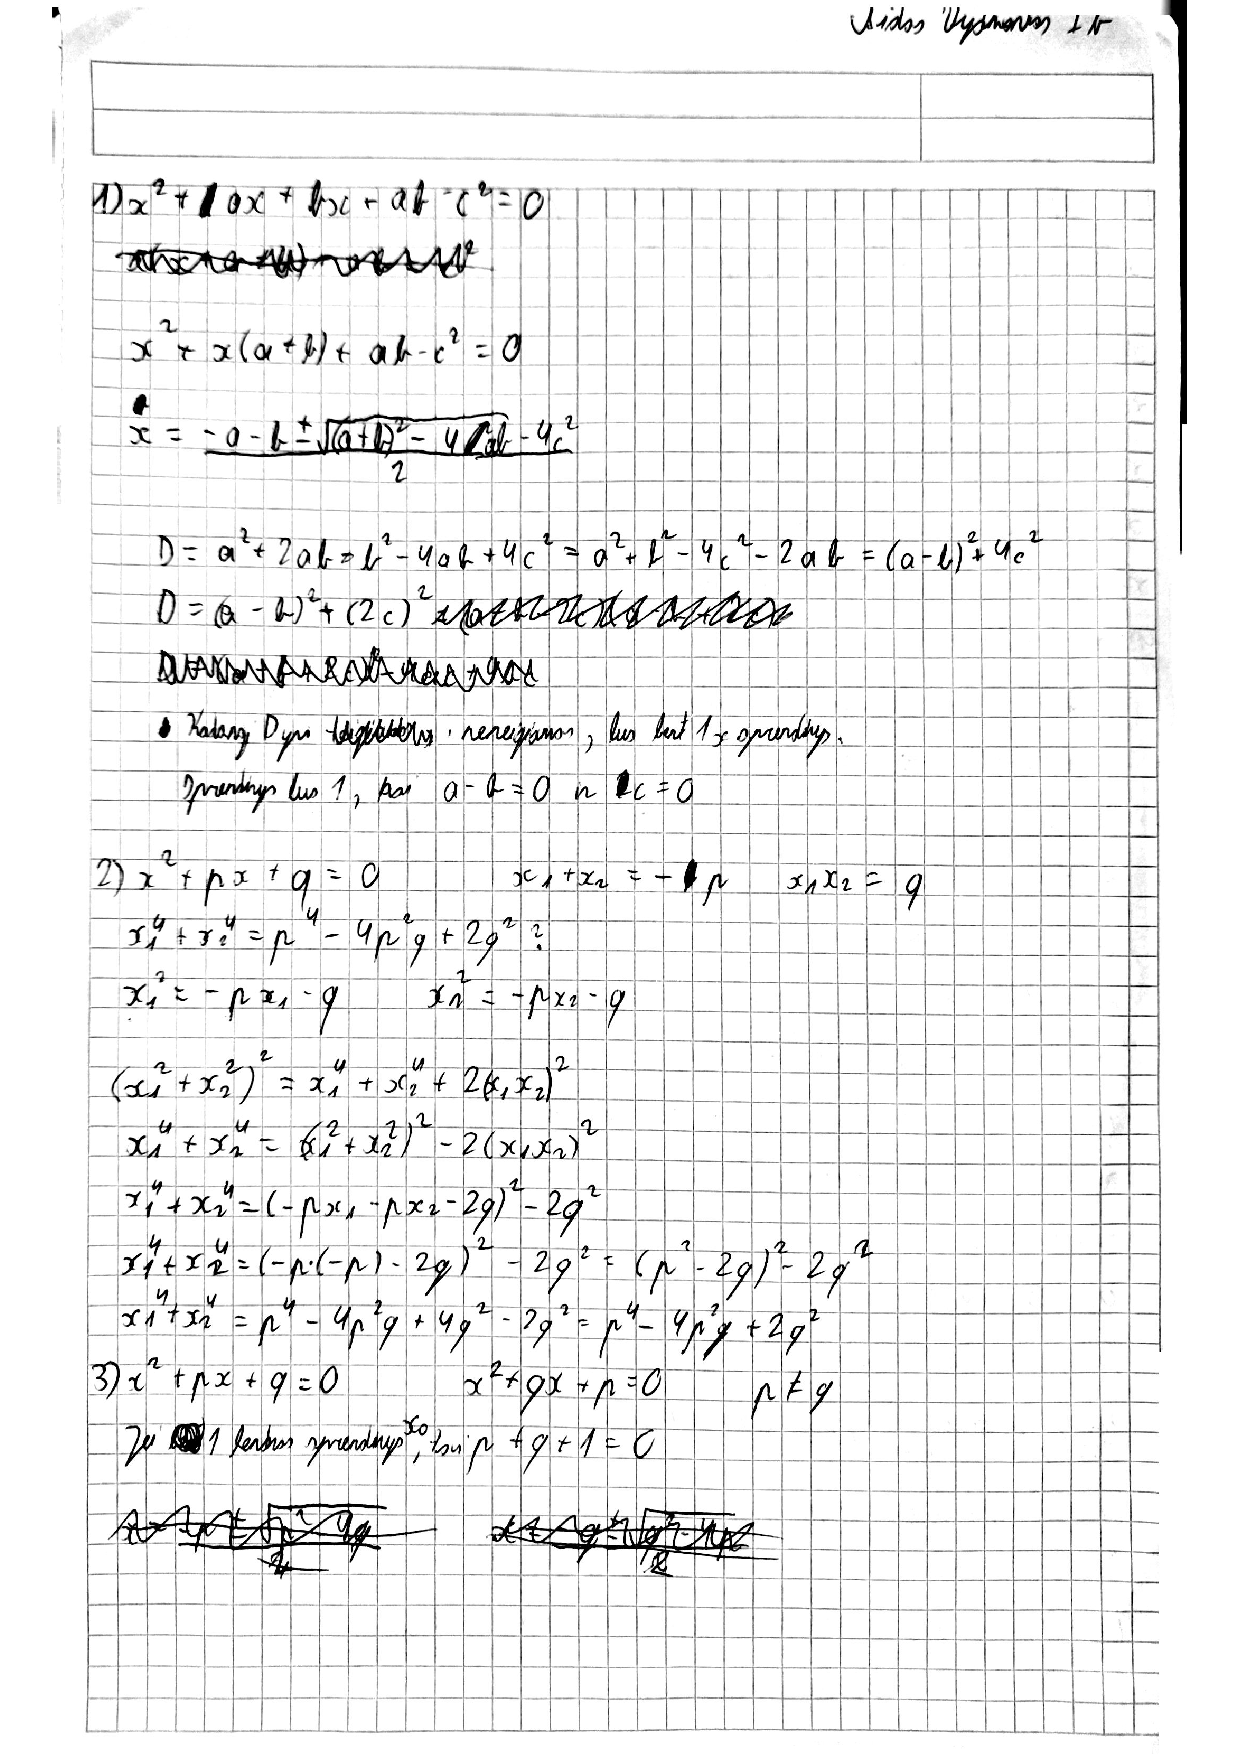
\includegraphics[page=1,trim={35.083 190.853 33.679 402.289},clip,width=\linewidth,height=.70\textheight,keepaspectratio]{Mokinio_originalas.pdf}\par
\end{center}
{\large\bfseries\color{ink}Pastabos ir pataisytas įrodymas}\par
\past
\begin{itemize}
\item Įžanga „Pagal Vijeto teoremą“ aiškiai įvardytų pirmųjų lygybių pagrindą. Toliau pakanka formulių.
\end{itemize}
\tais
Pagal Vijeto teoremą
\[
x_1+x_2=-p,\qquad x_1x_2=q.
\]
Kadangi $x_1$ ir $x_2$ yra duotosios lygties sprendiniai,
\[
x_1^2=-px_1-q,\qquad x_2^2=-px_2-q.
\]
Sudėję šias lygybes, gauname
\[
x_1^2+x_2^2=-p(x_1+x_2)-2q=p^2-2q.
\]
Naudodamiesi tapatybe
\[
(x_1^2+x_2^2)^2=x_1^4+x_2^4+2x_1^2x_2^2,
\]
gauname
\begin{align*}
x_1^4+x_2^4
&=(x_1^2+x_2^2)^2-2(x_1x_2)^2\\
&=(p^2-2q)^2-2q^2\\
&=p^4-4p^2q+4q^2-2q^2\\
&=p^4-4p^2q+2q^2.
\end{align*}
Taigi reikiama tapatybė įrodyta.\qed

\newpage
\uzd{3}{Lygtys $x^2+px+q=0$ ir $x^2+qx+p=0$, kur $p\ne q$, turi bendrą realųjį sprendinį. Įrodykite, kad $p+q+1=0$.}
\begin{center}
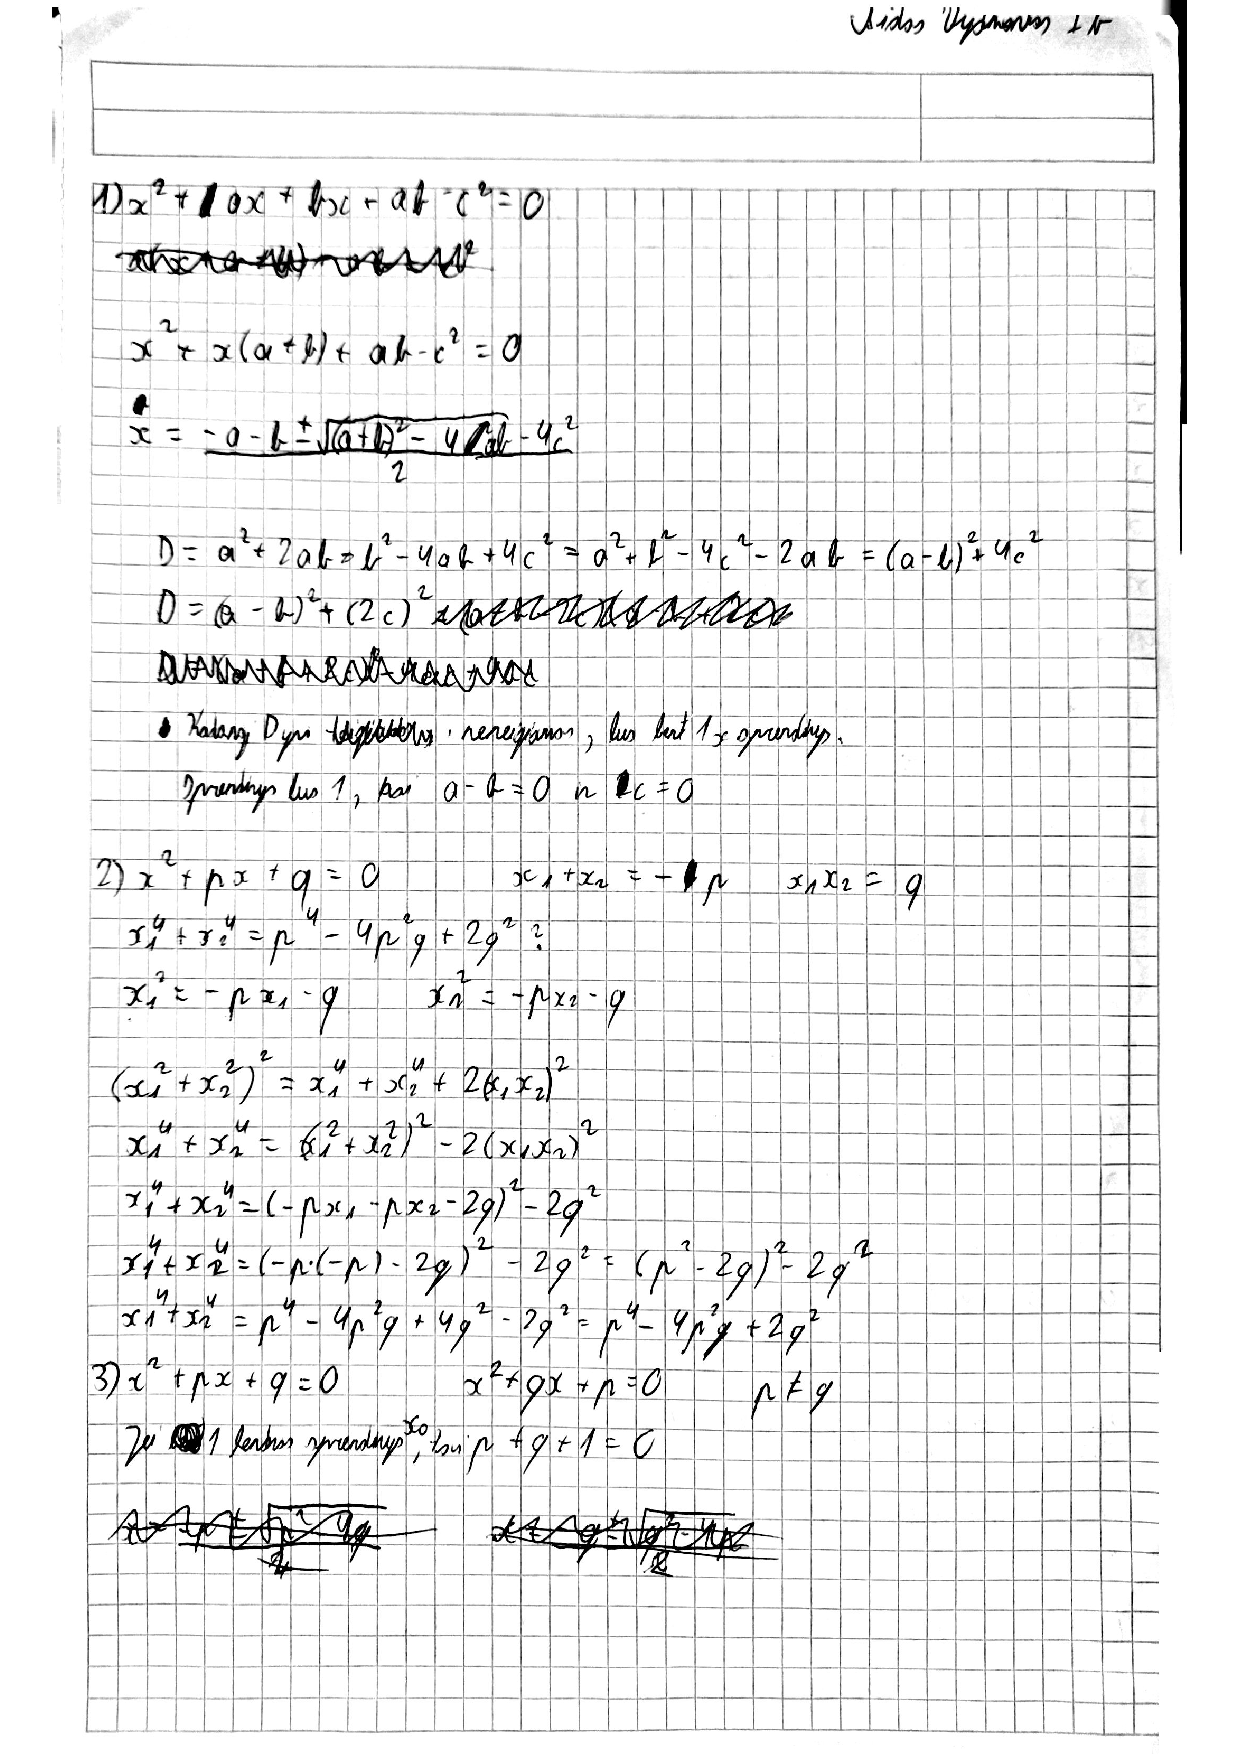
\includegraphics[page=1,trim={35.083 79.522 33.679 651.147},clip,width=\linewidth,height=.32\textheight,keepaspectratio]{Mokinio_originalas.pdf}\par
\includegraphics[page=2,trim={35.083 551.978 33.679 81.861},clip,width=\linewidth,height=.32\textheight,keepaspectratio]{Mokinio_originalas.pdf}\par
\end{center}
{\large\bfseries\color{ink}Pastabos ir pataisytas įrodymas}\par
\past
\begin{itemize}
\item Pirmiausia parašyti skliaustus saugiau negu iš karto išskleisti.
\item Prie išvados $x_0=1$ naudinga parašyti „Kadangi $p-q\ne0$“. Sąlyga jau duota, todėl tai išryškina pagrindą, o ne užpildo esminę naują spragą.
\end{itemize}
\tais
Tegu $x_0$ yra bendras abiejų lygčių realusis sprendinys. Tuomet
\[
x_0^2+px_0+q=0,\qquad x_0^2+qx_0+p=0.
\]
Atėmę antrąją lygybę iš pirmosios, gauname
\[
(x_0^2+px_0+q)-(x_0^2+qx_0+p)=0.
\]
Vadinasi,
\[
(p-q)x_0+q-p=0,
\qquad (p-q)(x_0-1)=0.
\]
Kadangi $p\ne q$, turime $p-q\ne0$. Todėl $x_0-1=0$, t.\,y. $x_0=1$.

Įstatę $x_0=1$ į pirmąją lygtį, gauname
\[
1+p+q=0.
\]
Taigi $p+q+1=0$, ką ir reikėjo įrodyti.\qed

\newpage
\uzd{4}{Lygtis $ax^2+bx+c=0$, kur $a>0$, neturi realiųjų sprendinių. Įrodykite, kad $a+b+c>0$.}
\begin{center}
\includegraphics[page=2,trim={35.083 294.700 33.679 292.361},clip,width=\linewidth,height=.70\textheight,keepaspectratio]{Mokinio_originalas.pdf}\par
\end{center}
{\large\bfseries\color{ink}Pastabos ir pataisytas įrodymas}\par
\past
\begin{itemize}
\item $b^2$ nebūtinai teigiamas: kai $b=0$, jis lygus nuliui. Reikia žodžio „neneigiamas“.
\item $c>0$ vis tiek išplaukia, nes $4ac>b^2\ge0$ ir $a>0$.
\item Aiškiai įvardytas $a>0$, $c>0$ pagrindžia šaknų $\sqrt a$, $\sqrt c$ vartojimą. 
\end{itemize}
\tais
Kadangi $a>0$, lygtis yra kvadratinė. Ji neturi realiųjų sprendinių, todėl jos diskriminantas neigiamas:
\[
b^2-4ac<0.
\]
Taigi $4ac>b^2\ge0$. Iš $a>0$ gauname $c>0$.

Kadangi $ac>0$ ir $b^2<4ac$, turime
\[
|b|<2\sqrt{ac},\qquad b>-2\sqrt{ac}.
\]
Todėl
\begin{align*}
a+b+c
&>a-2\sqrt{ac}+c\\
&=(\sqrt a-\sqrt c)^2\\
&\ge0.
\end{align*}
Vadinasi, $a+b+c>0$.\qed

\newpage
\uzd{5}{Lygčių $x^2+ax+b=0$ ir $x^2+cx+d=0$ koeficientai tenkina $ac=2(b+d)$. Įrodykite, kad bent viena lygtis turi realiųjų sprendinių.}
\begin{center}
\includegraphics[page=2,trim={35.083 21.050 33.679 549.639},clip,width=\linewidth,height=.70\textheight,keepaspectratio]{Mokinio_originalas.pdf}\par
\end{center}
{\large\bfseries\color{ink}Pastabos ir pataisytas įrodymas}\par
\past
\begin{itemize}
\item \textbf{Pagrindinė idėja tinkama:} diskriminantų suma leidžia panaudoti koeficientų sąryšį.
\item Teiginiai $a<0$, $c<0$ nepagrįsti. Pavyzdžiui, $a=c=2$, $b=d=1$ tenkina duotą sąryšį, nors $a,c>0$. 
\item Lygybė $a^2+c^2-2ac=(a+c)^2$ klaidinga. Teisingas kvadratas yra $(a-c)^2$.
\item Neneigiama suma neįrodo, kad abu diskriminantai neneigiami. Ji įrodo, kad bent vienas neneigiamas. Būtent šį tarpinį teiginį reikia susieti su sprendinių egzistavimu.
\end{itemize}
\tais
Pažymėkime pirmosios ir antrosios lygčių diskriminantus atitinkamai $D_1$ ir $D_2$. Tuomet
\[
D_1=a^2-4b,\qquad D_2=c^2-4d.
\]
Iš sąlygos $ac=2(b+d)$ gauname $4(b+d)=2ac$. Todėl
\begin{align*}
D_1+D_2
&=a^2+c^2-4(b+d)\\
&=a^2+c^2-2ac\\
&=(a-c)^2\ge0.
\end{align*}
Jeigu abu diskriminantai būtų neigiami, jų suma būtų neigiama. Tai prieštarauja gautai nelygybei. Vadinasi, bent vienas iš skaičių $D_1,D_2$ yra neneigiamas.

Abiejų lygčių vyriausiasis koeficientas lygus $1$. Todėl ta lygtis, kurios diskriminantas neneigiamas, turi bent vieną realųjį sprendinį. Taigi bent viena duotoji lygtis turi realiųjų sprendinių.\qed

\newpage
\uzd{6}{Kvadratinės lygties $ax^2+bx+c=0$, kur $a\ne0$, sprendiniai yra $x_1,x_2$, o $x_2=nx_1$. Įrodykite, kad $nb^2=(n+1)^2ac$.}
\begin{center}
\includegraphics[page=3,trim={46.777 308.733 33.679 77.183},clip,width=\linewidth,height=.70\textheight,keepaspectratio]{Mokinio_originalas.pdf}\par
\end{center}
{\large\bfseries\color{ink}Pastabos ir pataisytas įrodymas}\par
\past
\begin{itemize}
\item Dalijama iš $n$ ir $n+1$. Jei $n$ iš anksto laikomas teigiamu, dalybos leistinos. Tačiau vien lygybė $x_2=nx_1$ neatmeta $n=0$ ar $n=-1$.
\end{itemize}
\tais
Pagal Vijeto teoremą
\[
x_1+x_2=-\frac ba,\qquad x_1x_2=\frac ca.
\]
Kadangi $x_2=nx_1$, gauname
\[
(n+1)x_1=-\frac ba,\qquad nx_1^2=\frac ca.
\]
Pakėlę pirmąją lygybę kvadratu, turime
\[
(n+1)^2x_1^2=\frac{b^2}{a^2}.
\]
Padauginę ją iš $n$ ir panaudoję antrąją lygybę, gauname
\[
\frac{nb^2}{a^2}
=(n+1)^2nx_1^2
=(n+1)^2\frac ca.
\]
Padauginę iš $a^2$, gauname
\[
\boxed{nb^2=(n+1)^2ac.}
\]
Šis įrodymas nereikalauja prielaidų $n\ne0$ ar $n\ne-1$.\qed

\newpage
\uzd{7}{Įrodykite, kad jeigu $a,b,c$ yra nelyginiai sveikieji skaičiai, tai lygtis $ax^2+bx+c=0$ negali turėti sveikojo sprendinio.}
\begin{center}
\includegraphics[page=3,trim={46.777 58.472 33.679 533.267},clip,width=\linewidth,height=.70\textheight,keepaspectratio]{Mokinio_originalas.pdf}\par
\end{center}
{\large\bfseries\color{ink}Pastabos ir pataisytas įrodymas}\par
\past
\begin{itemize}
\item Abi parašytos sumų lyginumo taisyklės klaidingos. Lyginio ir lyginio suma lyginė; nelyginio ir nelyginio suma taip pat lyginė.
\item Jei užrašu norėjai parodyti neįmanomą lygybę tarp kairės ir dešinės pusių, reikia tai aiškiai atskirti nuo sumavimo taisyklės. Pirmiausia nustatyk kairės pusės lyginumą, tada palygink su $-c$.
\item Žodžių „tai neįmanoma“ neužtenka, jeigu neįvardyta, kas tiksliai prieštarauja kam.
\end{itemize}
\tais
Tarkime priešingai, kad egzistuoja sveikasis lygties sprendinys $x$. Tuomet
\[
ax^2+bx=-c.
\]
Kadangi $c$ nelyginis, $-c$ taip pat nelyginis. Nagrinėkime abu galimus sveikojo $x$ lyginumo atvejus.

\textbf{1 atvejis: $x$ lyginis.} Tada $x^2$ lyginis, todėl $ax^2$ ir $bx$ lyginiai. Jų suma $ax^2+bx$ lyginė.

\textbf{2 atvejis: $x$ nelyginis.} Tada $x^2$ nelyginis. Kadangi $a$ ir $b$ nelyginiai, sandaugos $ax^2$ ir $bx$ nelyginės. Dviejų nelyginių skaičių suma lyginė, todėl $ax^2+bx$ vėl lyginė.

Abiem atvejais lygybės $ax^2+bx=-c$ kairė pusė lyginė, o dešinė nelyginė. Tokia lygybė neįmanoma. Gavome prieštarą, todėl duotoji lygtis neturi sveikojo sprendinio.\qed

\newpage
\uzd{8}{Jeigu $p,q\in\mathbb Z$, o lygties $x^2+px+q=0$ diskriminantas yra sveikojo skaičiaus kvadratas, įrodykite, kad visi sprendiniai sveikieji.}
\begin{center}
\includegraphics[page=4,trim={35.083 500.522 33.679 79.522},clip,width=\linewidth,height=.70\textheight,keepaspectratio]{Mokinio_originalas.pdf}\par
\end{center}
{\large\bfseries\color{ink}Pastabos ir pataisytas įrodymas}\par
\past
\begin{itemize}
\item Užrašas $\sqrt{L-L}=L$ nėra pakankamas įrodymas. Pirmiausia reikia žinoti, kad šaknis sveikoji, tada pagrįsti ryšį tarp sveikojo skaičiaus ir jo kvadrato lyginumo.
\item Užbaik aiškiai: abu skaitikliai lyginiai, todėl abu dalmenys iš $2$ sveikieji. Atvejis $D=0$ taip pat įtrauktas.
\end{itemize}
\tais
Pagal sąlygą egzistuoja $m\in\mathbb Z$, kuriam $D=m^2$. Imkime $k=|m|\in\mathbb Z$, $k\ge0$. Tuomet
\[
k^2=D=p^2-4q.
\]
Kadangi $4q$ lyginis, skaičiai $k^2$ ir $p^2$ yra vienodo lyginumo.

Sveikasis skaičius ir jo kvadratas yra vienodo lyginumo: jei skaičius yra $2t$, jo kvadratas $4t^2$ lyginis; jei skaičius yra $2t+1$, jo kvadratas $4t^2+4t+1$ nelyginis. Todėl iš vienodo $k^2$ ir $p^2$ lyginumo išplaukia vienodas $k$ ir $p$ lyginumas.

Vadinasi, $-p+k$ ir $-p-k$ yra lyginiai sveikieji skaičiai. Kadangi $D=k^2\ge0$, visi lygties sprendiniai gaunami pagal kvadratinės lygties formulę:
\[
x_{1,2}=\frac{-p\pm\sqrt D}{2}=\frac{-p\pm k}{2}.
\]
Abu dalmenys sveikieji. Taigi visi lygties sprendiniai yra sveikieji skaičiai.\qed

\newpage
\uzd{9}{Jeigu $x^2+px+q=0$ turi realiųjų sprendinių, įrodykite, kad ir $x^2+px+q+\left(x+\frac p2\right)^2=0$ turi realiųjų sprendinių.}
\begin{center}
\includegraphics[page=4,trim={35.083 112.267 33.679 341.478},clip,width=\linewidth,height=.70\textheight,keepaspectratio]{Mokinio_originalas.pdf}\par
\end{center}
{\large\bfseries\color{ink}Pastabos ir pataisytas įrodymas}\par
\past
\begin{itemize}
\item Pataisytame variante verta pradėti diskriminantą nuo bendros išraiškos $(2p)^2-4\cdot2(q+p^2/4)$. Taip skaitytojui matyti, kad naudojami antrosios lygties koeficientai.
\item Nereikia papildomai skaičiuoti pačių šaknų: diskriminanto ženklo pakanka.
\item Nelygybė $D_2\ge0$ apima ir dvigubos šaknies atvejį.
\end{itemize}
\tais
Kadangi lygtis $x^2+px+q=0$ turi realiųjų sprendinių, jos diskriminantas tenkina
\[
D_1=p^2-4q\ge0.
\]
Išskleidę antrosios lygties kvadratą ir sutraukę panašiuosius narius, gauname lygiavertę lygtį
\[
2x^2+2px+q+\frac{p^2}{4}=0.
\]
Jos vyriausiasis koeficientas yra $2\ne0$, o diskriminantas
\begin{align*}
D_2
&=(2p)^2-4\cdot2\left(q+\frac{p^2}{4}\right)\\
&=4p^2-8q-2p^2\\
&=2(p^2-4q)\\
&=2D_1\ge0.
\end{align*}
Todėl antroji lygtis turi bent vieną realųjį sprendinį, ką ir reikėjo įrodyti.\qed

\newpage
\uzd{10}{Lygties $x^2-px+q=0$ sprendiniai $x_1,x_2$ yra teigiami realieji skaičiai. Remdamiesi diskriminantu įrodykite $p\ge2\sqrt q$.}
\begin{center}
\includegraphics[page=5,trim={35.083 540.283 33.679 79.522},clip,width=\linewidth,height=.70\textheight,keepaspectratio]{Mokinio_originalas.pdf}\par
\end{center}
{\large\bfseries\color{ink}Pastabos ir pataisytas įrodymas}\par
\past
\begin{itemize}
\item Reikia aiškiai pagrįsti ir $q>0$, kad $\sqrt q$ būtų realusis skaičius. Šį faktą tiesiogiai duoda teigiamų šaknų sandauga.
\item Pagal Vijeto teoremą galima iš karto pagrįsti abu ženklus. Diskriminantas ir toliau lieka pagrindinis reikiamos nelygybės argumentas, kaip prašoma sąlygoje.
\item Iš $p^2\ge4q$ pirmiausia gaunama $|p|\ge2\sqrt q$. Modulio atsisakoma tik žinant $p>0$.
\end{itemize}
\tais
Pagal Vijeto teoremą
\[
p=x_1+x_2,\qquad q=x_1x_2.
\]
Kadangi $x_1>0$ ir $x_2>0$, turime $p>0$ ir $q>0$.

Duotoji kvadratinė lygtis turi realiųjų sprendinių, todėl jos diskriminantas neneigiamas:
\[
D=(-p)^2-4q=p^2-4q\ge0.
\]
Vadinasi, $p^2\ge4q$. Abi pusės neneigiamos, todėl, pasinaudoję kvadratinės šaknies didėjimu, gauname
\[
\sqrt{p^2}\ge\sqrt{4q},\qquad |p|\ge2\sqrt q.
\]
Kadangi $p>0$, turime $|p|=p$. Taigi
\[
\boxed{p\ge2\sqrt q.}
\]
Reikiama nelygybė įrodyta.\qed

\vfill
\hrule
\medskip
\textbf{Bendra rašymo taisyklė.} Apibrėžk naujus žymėjimus, įvardykint atliekamus žingsnius, patikrink apribojimus ir užbaik tikslia išvada. Aiškių algebrinių veiksmų nereikia apkrauti komentarais.

\end{document}
